
For the last test case with known solution the method without additional gradient jump were did not work out just as in the test case before. We therefore only concentrate on the performances penalising the gradient jump across edges. The error made is to be found in figure \ref{fig: l2 errors test 3 jump} and table \ref{tab: l2 errors test 3 jump}. Again Newton's method did not converge for $k=3$, this time when refining the grid to $h=1/8$. 
\begin{figure}[H]
	\centering
	\begin{subfigure}{\textwidth}
		\centering
		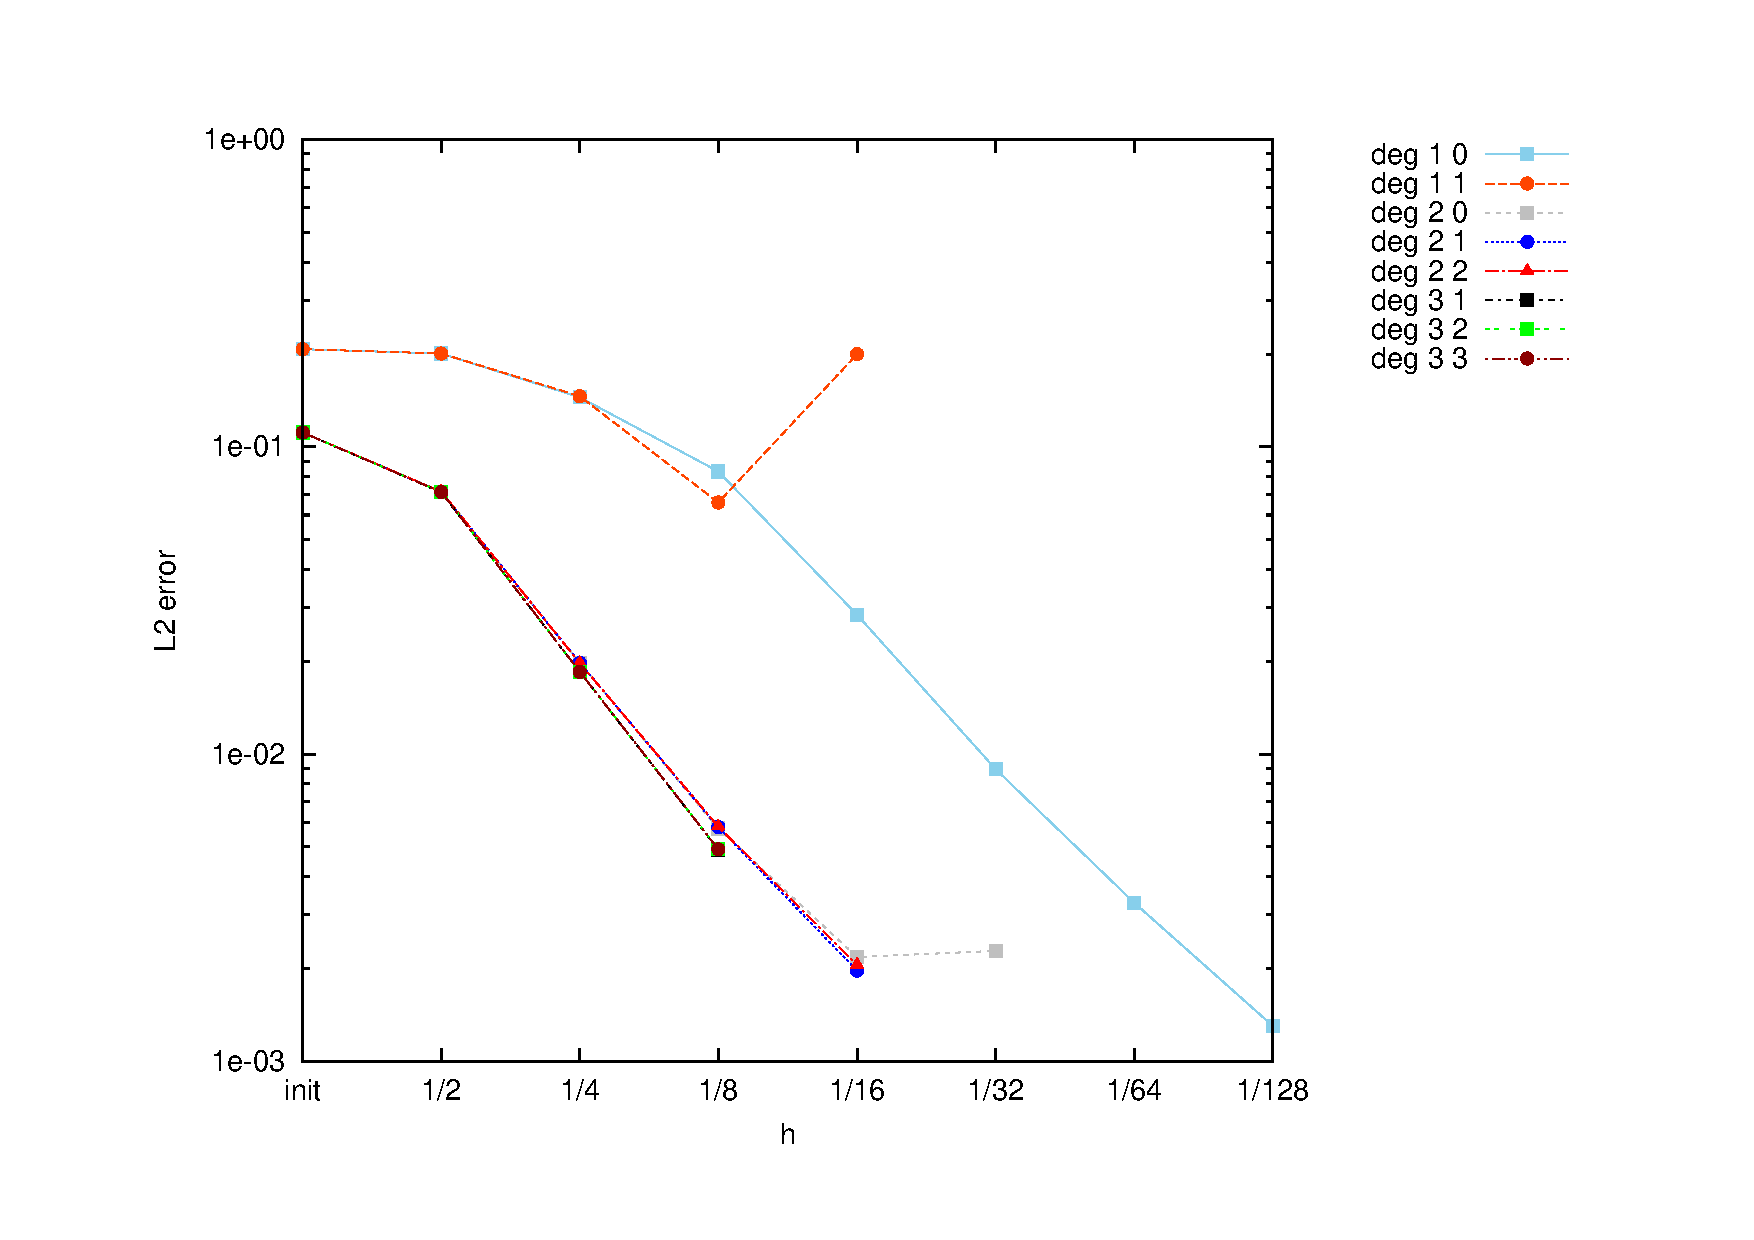
\includegraphics[scale =0.4]{../../FEniCS/diagrams/MA4_Neilan_GradJump_l2.pdf}
	\end{subfigure}
	
	\begin{subfigure}{\textwidth}
		\centering
		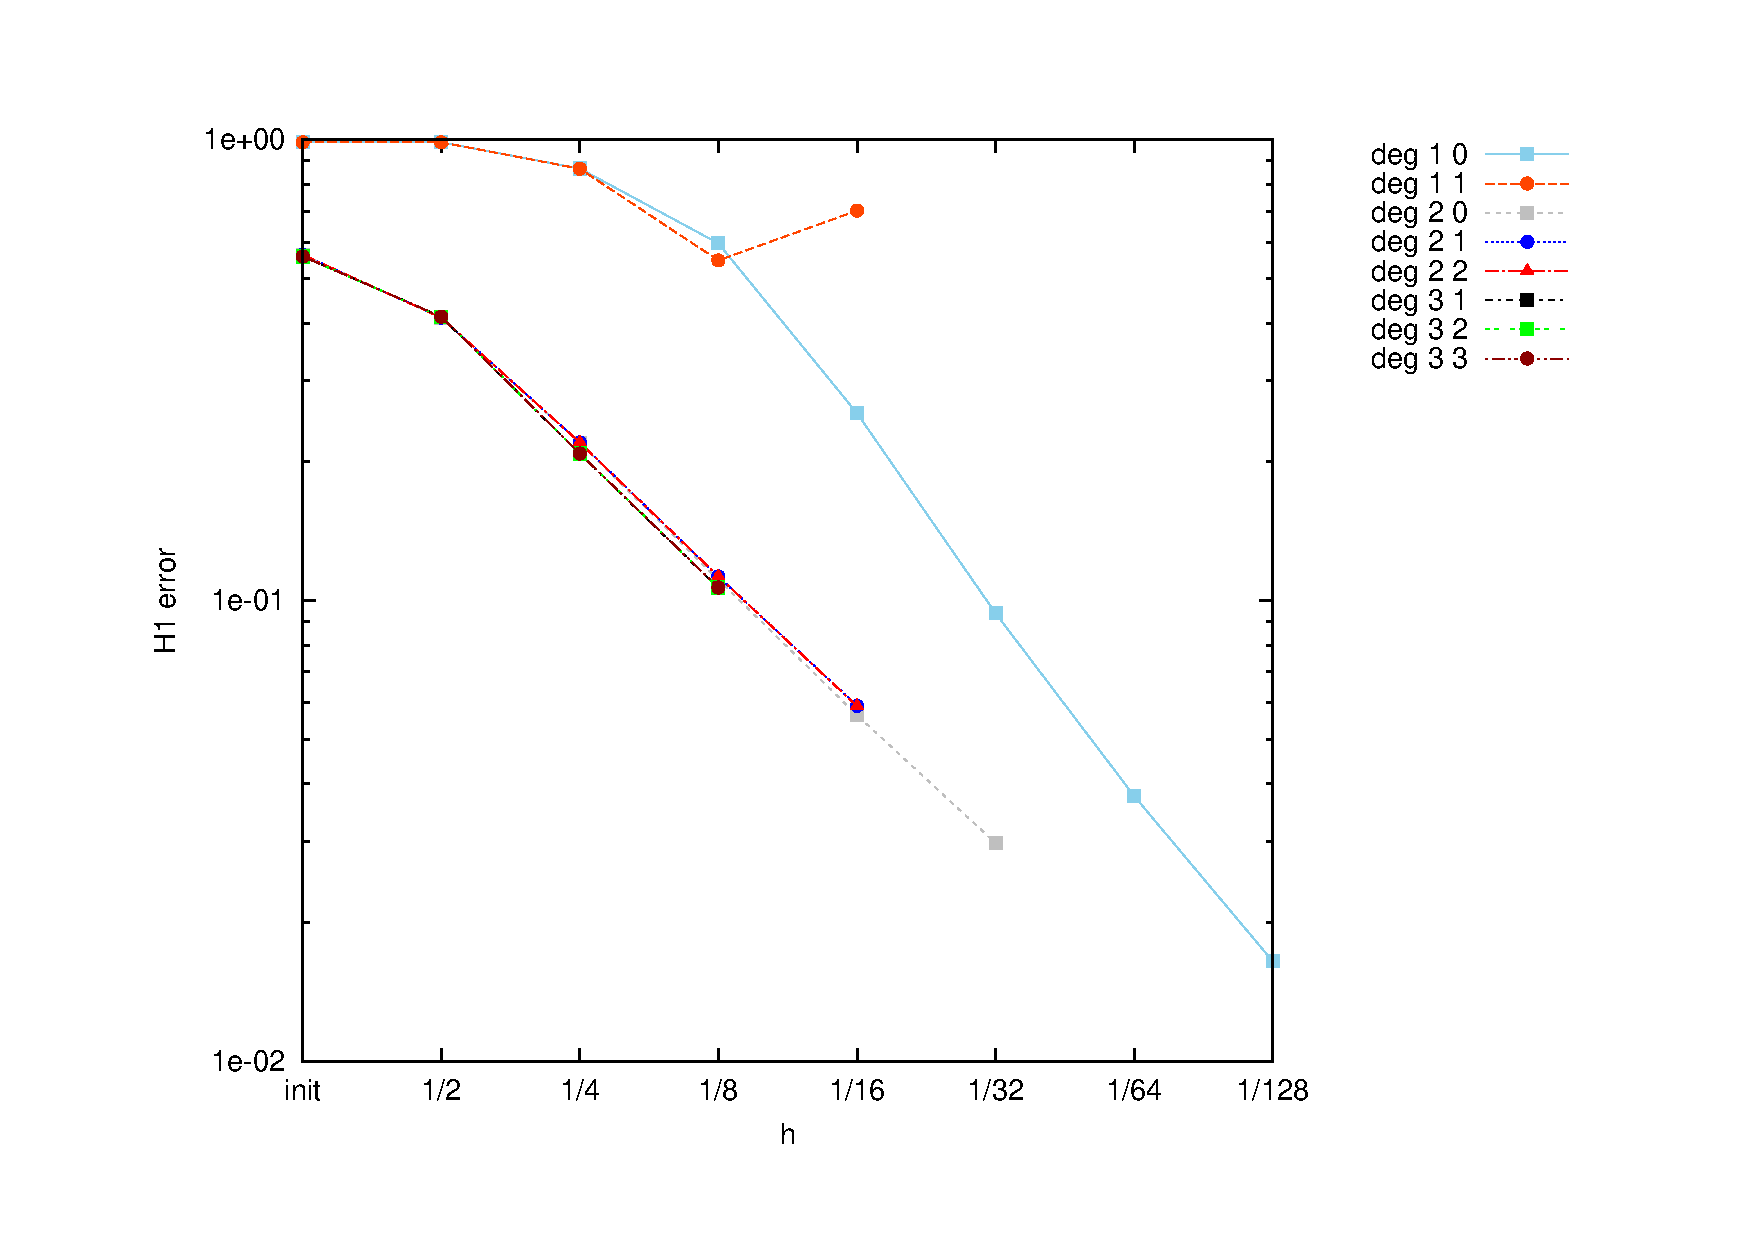
\includegraphics[scale =0.4]{../../FEniCS/diagrams/MA4_Neilan_GradJump_h1.pdf}
	\end{subfigure}
	\caption{$L^2$ and $H^1$ errors for test case \ref{test dirac} and additional gradient jump penalty}
	\label{fig: l2 errors test 4 jump}
\end{figure}
As before we do not experience much difference between the choices $k=2$ and $k=3$ during the first refinements. But as the Aleksandrov solution of this test case lacks regularity it is not surprising that decreasing the polynomial degree does not effect much the error made.

It is noticeable that for $k=2$ the $L^2$ error increases after four refinement while the $H^1$ error decreases. Table \ref{tab: l2 errors test 4 jump} states the results for $k=1, k_{DH}=0$ and $k=2, k_{DH}=2$. We see that it took the Newton solver 8 steps to converge in the last step which is twice as much as it needed in the case with $k=1$.
\begin{table}[H]
\begin{subtable}[b]{0.45\textwidth}
  	\centering
  	\pgfplotstabletypeset[columns={iterations, l2error, h1error,N},
  	every row 0 column 0/.style={set content=init},
  	]{\MAFourJumpdegOneZero}
  	\caption{Error for $k=1, k_{DH}=0$}
  \end{subtable}
  ~
	\begin{subtable}[b]{0.45\textwidth}
		\centering
		  		\pgfplotstabletypeset[
		columns={iterations, l2error, h1error,N},
		    every row 0 column 0/.style={set content=init},
		]{\MAFourJumpdegTwoTwo}
    	\caption{Error for $k=2, k_{DH}=2$}
   \end{subtable}
 	\caption{Errors for test case \ref{test dirac} and additional gradient jump penalty}
	\label{tab: l2 errors test 4 jump}
\end{table}
